\section{阻尼振动和$ Q $值}\label{sec:07.04}

简谐振动只是一种理想情况。因为我们在简谐振动中假定,
物体只受到弹性力(一种保守力)的作用,总机械能是保持不变
的。但在实际情况下,除去弹性力外,物体总还要受到阻力,例
如摩擦力的影响。在单摆摆动时,会受到空气的阻力。因而,实
际情况往往不是理想的简谐振动,振动物体的能量往往都会由于
阻力作用而不断减少。由于振动的能量和振幅平方成正比,所以
能量随时间减少时,振幅也就随时间衰减。

能量或振幅随时间衰减的振动过程称为阻尼振动。

图\ref{fig:07.08}给出了在阻尼振动过程中,位置$ x $和时间$ t $的典型关系。
在阻尼振动过程中,振幅由大变小,最后成为零,即振动停止。

为了描写阻力的影响,我们需要引进新的物理量。



% 207.jpg
\begin{figure}[t]
  \centering
  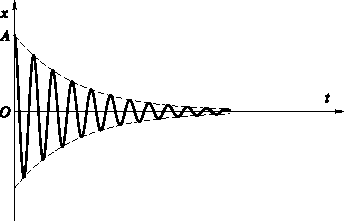
\includegraphics{figure/fig07.08}

  \caption{阻尼振动}
  \label{fig:07.08}
\end{figure}


由于阻力的存在,质点每完成一周期的振动,它的总能量$ E $中就有一部分消耗于克服阻力,用$ \left( \Delta E \right) _ { T } $表示示这个值。显然,
如果每周期消耗的能量$ \left( \Delta E \right) _ { T } $在总能量$ E $中占的份额越小,则表
示阻力越小,因而振动衰减越慢,越接近于理想简谐振动。这使
我们看到,可以用总能量$ E $与耗损能量$ \left( \Delta E \right) _ { T } $之比值$ \dfrac { E } { \left( \Delta E \right) _ { T } } $来作
为能量衰减的度量。通常,我们把比值$ \dfrac { E } { \left( \Delta E \right) _ { T } } $的$ 2 \uppi $倍定义为振
动系统的$ Q $值,也叫做品质因数,即
\begin{equation}\label{eqn:07.04.01}
  Q = 2 \uppi \frac { E } { \left( \Delta E \right) _ { T } }
\end{equation}
可见,$ Q $是无量纲的量。$ Q $越大,表示系统的阻尼损耗越小,衰减
越慢。当$ Q = \infty $时,就是理想的简谐振动情况

在阻尼振动过程中,$ E $是随时间变化的,$ \left( \Delta E \right) _ { T } $一般也随时
间变化,故由定义\lhbrak 式\ref{eqn:07.04.01}\rhbrak ,$ Q $可能是随时间变化的量。但是,
实际上有些阻尼振动过程一周期所“支出”的能量$ \left( \Delta E \right) _ { T } $与“库
存”的总能量$ E $成正比,$ E $越大,$ \left( \Delta E \right) _ { T } $也越大。在这种情况下,
$ Q $值与时间无关,是个常数。

现在我们讨论$ Q $为常数的阻尼振动的特征。我们知道,能量
% 208.jpg
对时间的微商$ \dif E / \dif t $代表单位时间内能量的增量。对于阻尼振动,

\clearpage\noindent
必定有$ \dif E / \dif t < 0 $,所以在一周期中能量的减少$ \left( \Delta E \right) _ { T } $应当是
\begin{equation*}
  \left( \Delta E \right) _ { T } = - \frac { \dif E } { \dif t } T
\end{equation*}
将上式代入式\eqref{eqn:07.04.01}中,整理后得
\begin{equation*}
  - \frac { \dif E } { \dif t } = \frac { 2 \uppi } { T } \cdot \frac { E } { Q }
\end{equation*}
又因$ \omega = \dfrac { 2 \uppi } { T } $,故有
\begin{equation}\label{eqn:07.04.02}
  - \frac { \dif E } { \dif t } = \frac { \omega E } { Q }
\end{equation}
式\eqref{eqn:07.04.02}是振动能量$ E $的微分方程。如果$ Q $是常数,很容易得到
上式的解为
\begin{equation}\label{eqn:07.04.03}
  E = E _ { 0 } \e ^ { - \frac { \omega } { Q } t }
\end{equation}
式中$ E _ { 0 } $是初始能量。可见,当$ Q $为常数时,阻尼振动能量随时间
作指数衰减,$ Q $越大,衰减越慢。$ Q $值的确描写了能量衰减的快
慢。

现在我们研究一个$ Q $为常数的实例。前面已经提到,单摆运
动要受到空气的阻力,阻力方向与质点速度方向相反,阻力大小
与速度值成正比。所以,空气阻力可以表示成
\begin{equation}\label{eqn:07.04.04}
  F _ { \text { 阻 } } = - \eta \frac { \dif x } { \dif t }
\end{equation}
其中系数$ \eta $标志阻力的大小。在水或其他液体中运动的物体所受
的阻力,也具有上述的形式。

阻力\lhbrak 式\eqref{eqn:07.04.04}\rhbrak 对质点作功,其功率由式\eqref{eqn:06.02.07}得
\begin{equation}\label{eqn:07.04.05}
  P = F _ { \text { 阻 } } \cdot \frac { \dif x } { \dif t } = - \eta \left( \frac { \dif x } { \dif t } \right) ^ { 2 }
\end{equation}
% 209.jpg
这个功率就应当等于质点能量的减少率。

注意到式\eqref{eqn:07.02.07},上式可以写成
\begin{equation*}
  P = - \eta \omega ^ { 2 } A ^ { 2 } \sin ^ { 2 } \left( \omega t + \varphi _ { 0 } \right)
\end{equation*}
在一个周期的时间里,阻力作功的数值等于
\begin{equation}\label{eqn:07.04.06}
  \begin{aligned}
    \Delta A & = \int _ { 0 } ^ { T } P \dif t                                                                                      \\
             & = - \eta \omega ^ { 2 } A ^ { 2 } \int _ { 0 } ^ { T } \sin ^ { 2 } \left( \omega t + \varphi _ { 0 } \right) \dif t \\
             & = - \uppi \eta \omega A ^ { 2 }
  \end{aligned}
\end{equation}
$ - \Delta A $就是在一个周期的时间里,振子损失的能量。即
\begin{equation*}
  \left( \Delta E \right) _ { T } = - \Delta A
\end{equation*}
再注意到式\eqref{eqn:07.02.05},则由式\eqref{eqn:07.04.06}可推得
\begin{equation}\label{eqn:07.04.07}
  Q = \frac { 2 \uppi E } { \left( \Delta E \right) _ { T } } = \frac { k } { \eta \omega } = \frac { \sqrt { k m } } { \eta }
\end{equation}
最后一步利用$ \omega ^ { 2 } = k / m $。因$ m $及$ \eta $都是常数,所以现在品质因数$ Q $
也是一个常数。

在有阻力\lhbrak 式\eqref{eqn:07.04.04}\rhbrak 的情况下,振子的运动方程为
\begin{equation*}
  m \frac { \dif ^ { 2 } x } { \dif t ^ { 2 } } = - k x - \eta \frac { \dif x } { \dif t }
\end{equation*}
或
\begin{equation*}
  \frac { \dif ^ { 2 } x } { \dif t ^ { 2 } } + \frac { \eta } { m } \cdot \frac { \dif x } { \dif t } + \frac { k } { m } x = 0
\end{equation*}
令$ \omega _ 0 ^ { 2 } = \dfrac { k } { m } $, $ \beta = \dfrac { \eta } { 2 m } $,则有
\begin{equation}\label{eqn:07.04.08}
  \frac { \dif ^ { 2 } x } { \dif t ^ { 2 } } + 2 \beta \frac { \dif x } { \dif t } + \omega _ { 0 } ^ { 2 } x = 0
\end{equation}
这就是阻尼振动的基本方程。当$ \beta < \omega _ { 0 } $时,它的解为
\begin{equation}\label{eqn:07.04.09}
  x = A _ { 0 } \e ^ { - \beta t } \cos \left( \omega t + \varphi _ { 0 } \right)
\end{equation}
其中$\omega = \sqrt { \omega _ 0 ^ { 2 } - \beta ^ { 2 } } $, 式\eqref{eqn:07.04.09}是阻尼振动的振动解,与理想的
简谐振动相比较,它只多了一个因子$ \e ^ { - \beta t } $,这表示振幅是以指数形
% 210.jpg
式衰减的。式\eqref{eqn:07.04.09}的$ x \mathdash t $曲线,即有图\ref{fig:07.08}的形式。另外应注意
到,阻力不仅对振幅有影响,而且也影响到周期。当$ \beta = 0 $时,振
动周期为$ T = \dfrac { 2 \uppi } { \omega _ { 0 } } $;$ \beta \ne 0 $有阻力时,周期变为
$ T = \dfrac { 2 \uppi } { \sqrt { \omega _ { 0 } ^ { 2 } - \beta ^ { 2 } } } $
即阻力的存在使周期变长。若阻力很大$ \beta \to \omega _ { 0 } $,则周期$ T \to \infty $。这
就是说,如果阻力太大,质点的周期振动将消失。因此,为了消
除一些不必要的振动,可以采用增加阻力的办法。
